\chapter{Pear区块链方案}

Pear在自主创新的基础上,打造了提供企业级服务“Pear区块链”解决方案。基于“开放包容”的理念,Pear将搭建区块链基础设施,并开放内部能力,与合作企业共享,共同推动共享经济的发展,打造区块链的共赢生态。\par 
Pear是第一个提出“共享雾计算”技术并将其落地实现的创新型企业,成功开发了第一个建立在智能路由器、NAS、浏览器之上的众包共享雾计算平台,从海量、分布式的节点中构建起安全可靠、Web友好的边缘网络,共享边缘设备的带宽、存储、计算资源。
\section{设计原则及目标}
Pear区块链致力于提供企业级区块链基础设施,行业解决方案,以及安全、可靠、灵活的区块链雾服务。
\subsection{设计原则}
\textbf{融合创新:}  Pear区块链注重融合创新,将区块链技术融入到共享经济体系中,致力于推动发展新型的共享理念,同时共享理念的散播也推动着“多极”区块链的发展。\par 
\textbf{安全可靠:} Pear区块链对区块链底层的算法进行优化,提升其运行效率以及安全性,保证共享信息的安全可靠。\par 
\textbf{开放包容:}
Pear负责搭建共享雾计算的基础设施,开放内部服务能力,任何愿意与Pear合作的厂商可以接入Pear搭建的区块链平台,共建共享、区块链生态。

\subsection{设计目标}
Pear区块链旨在为行业伙伴提供企业级区块链基础设施,行业解决方案,以及安全、可靠、灵活的区块链雾服务。通过高性能的区块链服务,在实现安全可靠的对接的前提下,帮助企业具有区块链雾服务能力,在其硬件平台上运行Pear雾服务,实现多方共赢。

\section{Pear区块的整体架构}
在“融合创新、安全可靠、开放包容”设计原则的指导下,Pear区块链方案的整体架构分为三个层次:Pear区块链的底层是Pear自主研发的Fog API,通过API接口为上层应用场景提供区块链基础服务功能,中间是平台产品服务层为Fog Platform,在底层(Fog API)之上构建高可用性,可扩展性的区块链基础平台,帮助企业方便使用Pear Fog服务的底层接口。此次开放的为Fog API以及Fog Platform,第三个层次Fog Application 不在Pear的提供解决方案内。Fog Application 为最终向用户提供基于Pear Fog底层服务开发的应用,因现阶段种种限制因素,将开放给所有与Pear合作的厂商进行开发,共同探索行业区块链的发展方向,共同推进区块链应用场景落地,整体框架结构如下图:
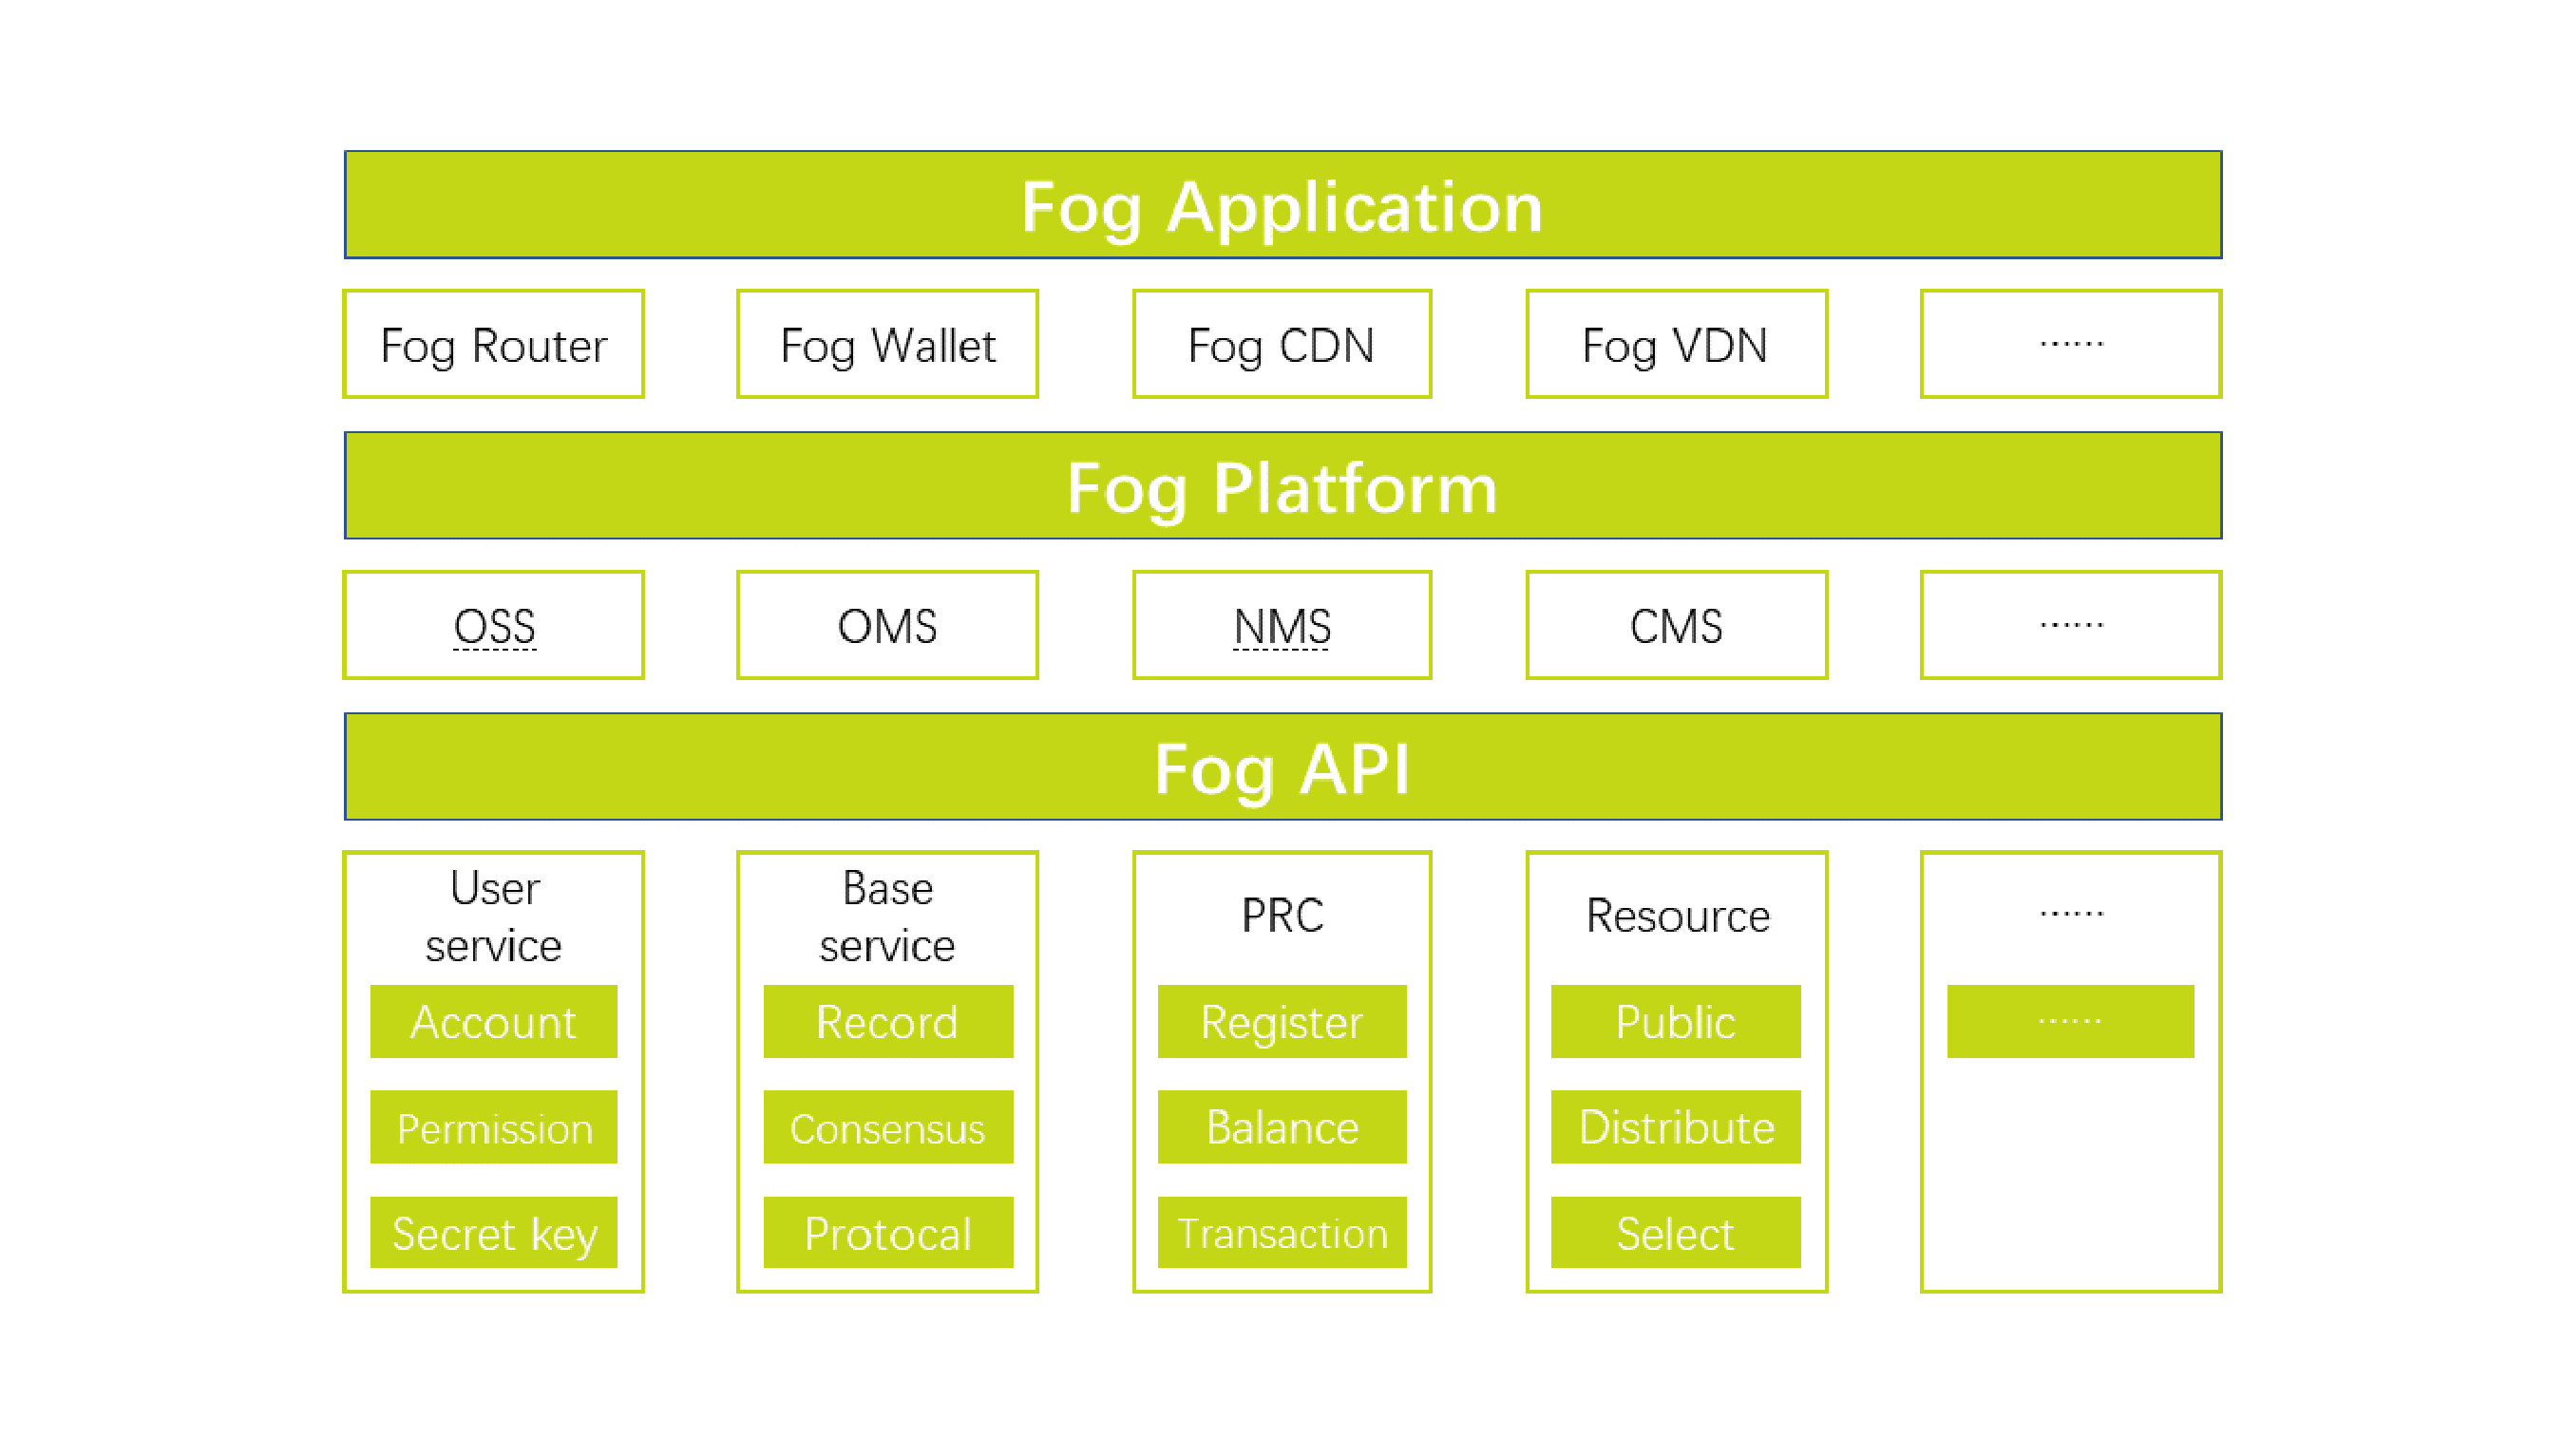
\includegraphics[width= 6.5 in]{frame.eps}



\section{接入Pear区块链的基本要求}
\subsection{系统硬件最低要求}
\begin{table}[!htb] 
\Large    
\begin{center}  
\begin{tabular}{|l|l|}  
\hline  
主频 & 880Mhz\\ \hline  
内存  & 512M \\ \hline  
flash& 32M\\ \hline
支持USB3.0& 是 \\ \hline
I/O & 25MB/s \\ \hline
预留系统空间&12M \\ \hline
\end{tabular}  
\end{center}  
\end{table}  
\subsection{系统软件要求}
操作系统,推荐为OpenWrt, Ubuntu, 类Linux系统 \par 
支持文件系统:ext3/4, FAT32, exFAT 



